\documentclass[conference]{IEEEtran}
\usepackage{amsmath,amssymb}
\usepackage{graphicx}
\usepackage{booktabs}
\usepackage{xcolor}
\usepackage{url}
\usepackage[hidelinks]{hyperref}
\graphicspath{{../results/}}

\begin{document}

\title{Probabilistic Prediction of Outcome and Herding Time in Single-Pursuer Multi-Evader Herding}

\author{\IEEEauthorblockN{Shreyas Reddy Duggimpudi (EC24BT033)}
\IEEEauthorblockA{EE604T Pattern Recognition and Machine Learning, IIT Dharwad}}

\maketitle

\begin{abstract}
A single pursuer can herd many non-cooperative evaders by circling a goal with a radius that follows one tracked
evader. Existing theory for this law is local: it guarantees a stable herd near the equilibrium but says nothing
about which starting configurations end in success, in a stalled herd, or in a lost evader, or how long herding
takes. We learn this map from 60{,}000 validated simulations with classical, probabilistic machine learning.
A Gaussian-process (GP) classifier on permutation-invariant features predicts the three-way outcome from the start
alone with 93.7\,\% balanced accuracy and the best calibrated probabilities of all models, and reveals that
evaders are lost even where the stability condition of the theory holds; a set kernel keeps 93.8\,\% on flock sizes
never seen in training. A kernel mixture-cure survival model separates slow from stuck herds beyond the simulation
horizon (AUC 0.98 against ten-times-longer re-simulation). A risk-aware active-learning rule that picks the next
simulation by the Bayes risk of the decision reaches the decision cost of random sampling with 2.3$\times$ fewer
simulations, whereas entropy sampling worsens it. Used to choose the pursuer settings, the risk-aware model matches the
theory-guided rule's zero losses while herding 2.3$\times$ faster in simulation.
\end{abstract}

\section{Introduction}
Herding many evaders with one pursuer is a hard nonlinear, switched-like control problem. Singh and Chakraborty
proposed a circular pursuer trajectory~\cite{singh2024cdc} and a feedback variant whose radius follows the evader
that was farthest at the start~\cite{singh2025arxiv}. Their theorems give existence, uniqueness and local
asymptotic stability of a common equilibrium ring under a parameter condition, and an inner (Lyapunov-ellipse)
estimate of the region of attraction for the tracked evader. For the other evaders, the region is only shown by
brute-force simulation~\cite{singh2025arxiv}.

A practitioner needs more: \emph{given this flock and these settings, will herding succeed, stall, or lose an evader,
how sure are we, and how long will it take?} We treat this as a pattern-recognition problem. Contributions:
\begin{enumerate}
\item A validated dataset and calibrated probabilistic predictors (GP classification and regression, Bayes-risk
decisions) of the outcome and herding time for any flock size, with an analysis of where the local theory fails.
\item A kernel mixture-cure survival model for herding time with right-censoring, which separates slow herds from
herds that never settle.
\item Risk-aware active learning: choosing the next simulation by the Bayes risk of the downstream decision, and the
finding that the usual uncertainty-based choice optimises the wrong target.
\item A set kernel (kernel mean embedding) over the evaders that generalises to unseen flock sizes, and a
risk-aware choice of pursuer settings validated by simulation against a theory-guided rule.
\end{enumerate}
GP classification with active learning has estimated regions of attraction of single systems~\cite{wang2023roa}
and missile capture regions~\cite{lee2022capture}; see also safe ROA learning~\cite{berkenkamp2016}. We add three
asymmetric-cost outcome classes, many agents with permutation-invariant inputs, censored times, and a decision-driven
acquisition rule.

\section{Related Work}
\emph{Herding.} The circular law~\cite{singh2024cdc} yields a stable and an unstable limit cycle and an inner Lyapunov
estimate of the region of attraction (ROA); the feedback law~\cite{singh2025arxiv} adds a unique, locally stable
common equilibrium for all evaders when $2k_1^2R^2>1$ and $\kappa<\ln(2k_1^2R^2)/(2k_1)$. Global behaviour, losses and
herding time are not characterised.
\emph{Learning ROAs.} GP classification estimates ROAs with confidence and active learning~\cite{wang2023roa}, and
missile capture regions with uncertainty sampling~\cite{lee2022capture}; GP-based safe exploration learns ROAs of
uncertain systems~\cite{berkenkamp2016}. Classical Lyapunov estimates~\cite{khalil2002,davison1971} are sound but can be
conservative; we quantify how much.
\emph{Survival models.} Tobit regression~\cite{tobin1958} handles censoring; mixture-cure models~\cite{farewell1982} add a
sub-population that never experiences the event. We use kernel versions via random features~\cite{rahimi2007rff}.
\emph{Active learning}~\cite{settles2009} usually targets uncertainty; we target the Bayes risk of the decision.

\section{System and Data}
\subsection{Model}
Evader $i$ at $x_i\in\mathbb{R}^2$ moves away from the pursuer $p$ with speed $k/d_i^2$, $d_i=\|x_i-p\|$; evaders do
not interact~\cite{singh2024cdc}. The pursuer moves at angular speed $\omega$ with radius
$R_p(t)=R\,e^{k_1(r_0(t)-\kappa)}$, where $r_0$ is the distance of the tracked evader (farthest at $t=0$) and
$\kappa=r_0(0)$~\cite{singh2025arxiv}; $k_1=0$ gives the fixed circle of~\cite{singh2024cdc} (our baseline law).
In the frame rotating with the pursuer the dynamics are autonomous. Scaling lengths by $1/k_1$ and time by $1/\omega$
leaves two parameters, $q=k_1R$ and $\beta=k k_1^3/\omega$, plus the scaled start; for the circle law only
$\gamma=k/(\omega R^3)$ remains. The theory's condition is $a=2q^2e^{-2\kappa}>1$ (in scaled units).

\subsection{Labels}
A run is \emph{loss} if an evader leaves the pursuer circle at $T_{\max}=300$ laps or goes beyond an escape radius;
\emph{success} if, from some lap $t_s$ on, every evader stays within 1\,\% (radius) and $0.05$\,rad of the common
equilibrium; otherwise \emph{deadlock}. The herding time is $T_h=t_s$.

\subsection{Simulation and data}
We wrote our own simulator (RK4 with a step that shrinks during close passes). It reproduces the published ring
radii~\cite{singh2024cdc}, the equilibrium of the running example of~\cite{singh2025arxiv}, an independent
loss count for the tracked-index law, and agrees with an adaptive DOP853 solver: 700 of 700 re-simulated runs get the
same label and herding time. We generated 60{,}000 arXiv-law runs ($N=1..6$, three strata of $a$: $a>1$,
$6/e^2<a\le1$, $a\le6/e^2$; Latin-hypercube sampling~\cite{mckay1979}; plus boundary sets) and 10{,}000 circle-law
runs: 26{,}454 success, 16{,}013 deadlock, 17{,}533 loss. A fixed stratified 20\,\% test set is used throughout.

\subsection{Features}
Only the start is used. Lengths are divided by $\kappa$. Global: $N$, $\log q$, $\log\beta$, $\kappa$, $\log a$,
$\log(q/\kappa)$, $\log(r^*/\kappa)$. Flock: means, spreads and minima of radii, circular variance, largest angular
gap, pairwise distances, hull area, angles relative to the pursuer and to the tracked evader, distances to the
pursuer and to the equilibrium point. All are permutation-invariant and defined for every $N$ (24 features).

\section{Methods}
\subsection{Classifiers and calibration}
Baselines: majority class, the theory rule (success iff $a>1$), logistic regression, and an RBF-SVM (with Platt
scaling~\cite{platt1999} for probabilities). The GP classifier uses one binary GP per class (Laplace approximation,
one-vs-rest~\cite{rasmussen2006gpml}) with an ARD kernel $\sigma_f^2\exp(-\tfrac12\sum_j (x_j-x'_j)^2/\ell_j^2)$.
Exact GP cost is $O(n^3)$, so the kernel is tuned by marginal likelihood on 1{,}000 runs and the GP is fitted on
4{,}000. We cap $\sigma_f^2\le100$: without the cap, three of six random training sets produced an over-confident
GP (balanced accuracy down to 0.885); with it, seven sets give 0.936--0.938.

\subsection{Bayes-risk decisions}
With cost matrix $L$ (calling a true loss ``success'' costs 10; loss$\to$deadlock and deadlock$\to$success cost 3;
other errors 1), the decision is $\hat a(x)=\arg\min_j \sum_i P(i\mid x)\,L_{ij}$.

\subsection{Herding time with censoring}
Let $y=\log(1+T_h)$ and $c=\log(1+T_{\max})$. With random Fourier features $z(x)$~\cite{rahimi2007rff} of the ARD
kernel, $f(x)=b+w^\top z(x)$ approximates a GP. The Tobit model~\cite{tobin1958} uses $y\sim\mathcal{N}(f,\sigma^2)$
for settled runs and $P(y>c)=\Phi((f-c)/\sigma)$ for deadlocks. Our \emph{kernel mixture-cure} model~\cite{farewell1982}
adds $\pi(x)=\mathrm{sigmoid}(g(x))$, the probability that a run ever settles:
\begin{equation}
\mathcal{L}=\prod_{\text{settled}} \pi\,\mathcal{N}(y;f,\sigma^2)\prod_{\text{deadlock}}\big[(1-\pi)+\pi\,\Phi(\tfrac{f-c}{\sigma})\big],
\end{equation}
with Gaussian priors on the feature weights (MAP by L-BFGS with analytic gradients).

\subsection{Risk-aware active learning}
Starting from 200 random runs, the GP repeatedly adds batches from a pool. \emph{Entropy} sampling picks the largest
predictive entropy~\cite{settles2009}. \emph{Risk-aware} sampling picks the largest Bayes risk of the best decision,
$r(x)=\min_j\sum_i P(i\mid x)L_{ij}$, i.e.\ where acting is most expensive.

\subsection{Evaluation protocol}
All models share one fixed, stratified (label $\times N$) 20\,\% test set (12{,}000 runs) that is never used for tuning;
settings are chosen by cross-validation on training data only. We report balanced accuracy (mean per-class recall),
log-loss, Brier score and expected calibration error (ECE, 15 bins); for times, median error and interval coverage;
for censored times, the time-dependent concordance $C_{td}$~\cite{antolini2005}. Paired comparisons on the same flocks
use exact McNemar and Wilcoxon signed-rank tests. Every learned conclusion that matters is checked by new simulations.

\section{Results}
\subsection{Outcome prediction}
\begin{table}[t]
\centering
\caption{Test-set results (12{,}000 runs). Bal.\ acc.\ = mean per-class recall.}
\label{tab:cls}
\begin{tabular}{lcccc}
\toprule
model (training runs) & bal.\ acc. & log-loss & Brier & ECE\\
\midrule
theory rule ($a>1$) & 0.457 & -- & -- & --\\
logistic regression (48k) & 0.825 & 0.482 & 0.258 & 0.039\\
SVM + Platt (4k) & 0.918 & 0.254 & 0.130 & 0.034\\
SVM + Platt (20k) & 0.938 & 0.200 & 0.099 & 0.021\\
GP classifier (4k) & 0.937 & \textbf{0.162} & \textbf{0.092} & 0.028\\
\bottomrule
\end{tabular}
\end{table}
Table~\ref{tab:cls}: the GP matches the SVM trained on five times more data in accuracy and gives the best
probabilities. Trained on $N\le4$ and tested on $N=5,6$, the SVM keeps 92.8\,\%. The theory rule reaches only
45.7\,\%: 52\,\% of successful runs violate $a>1$ and 11\,\% of lost runs satisfy it. Uncertainty is informative:
answering only the 80\,\% most confident runs raises GP accuracy to 98.6\,\%. The Bayes rule cuts ``loss called
success'' from 169 to 9 test runs. Fig.~\ref{fig:map} compares the learned map with 1{,}600 fresh simulations
(97.3\,\% agreement): losses occur right of $a=1$, where the theorems hold, because those theorems are local.
\begin{figure*}[t]
\centering
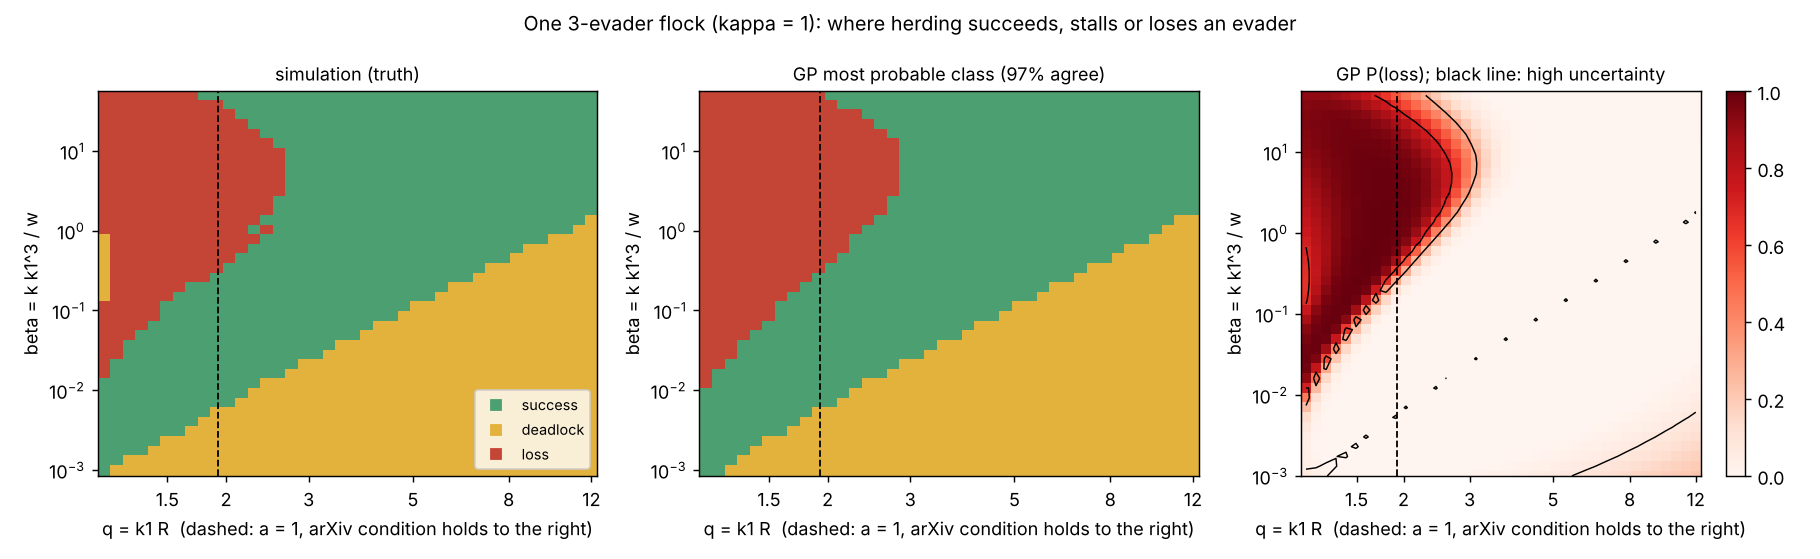
\includegraphics[width=0.92\textwidth]{phase3/map.png}
\caption{One 3-evader flock: simulated outcome (left), GP prediction (middle) and GP $P(\text{loss})$ with its
high-uncertainty contour (right) over $q$ and $\beta$; dashed: $a=1$.}
\label{fig:map}
\end{figure*}

\subsection{Herding time}
On settled test runs a GP regression predicts $T_h$ with median error 0.7 laps and 89\,\% coverage of its 90\,\%
bands, but it ignores the 27\,\% of runs that stop unsettled at $T_{\max}$. Table~\ref{tab:cens} compares three
censoring-aware variants sharing the same RFF kernel (1{,}000 features). The mixture-cure model is best on every test
measure. The decisive check goes beyond the training horizon: 300 test deadlock runs re-simulated $10\times$ longer
(3{,}000 laps) split into 158 that settle, 137 that never do and 5 losses. From the start alone the cure model
predicts which ones settle with AUC 0.984 and Brier 0.049 (Tobit 0.216, successes-only 0.345); its mean predicted
probability, 0.535, matches the observed 0.536, and it predicts their herding times within a median factor of 1.09
(Fig.~\ref{fig:cens}). ``Deadlock'' thus hides two regimes, slow and stuck, which the model separates.
\begin{table}[t]
\centering
\caption{Censored herding time on the test set (settled and deadlock runs).}
\label{tab:cens}
\begin{tabular}{lccc}
\toprule
 & successes only & Tobit & cure\\
\midrule
log-likelihood / run & $-24.05$ & $-0.27$ & $\mathbf{+0.37}$\\
time concordance $C_{td}$~\cite{antolini2005} & 0.943 & 0.979 & \textbf{0.992}\\
settled: median error (laps) & 0.72 & 1.95 & \textbf{0.69}\\
deadlock: mean $P(T_h>T_{\max})$ & 0.83 & 0.95 & \textbf{0.98}\\
\bottomrule
\end{tabular}
\end{table}
\begin{figure}[t]
\centering
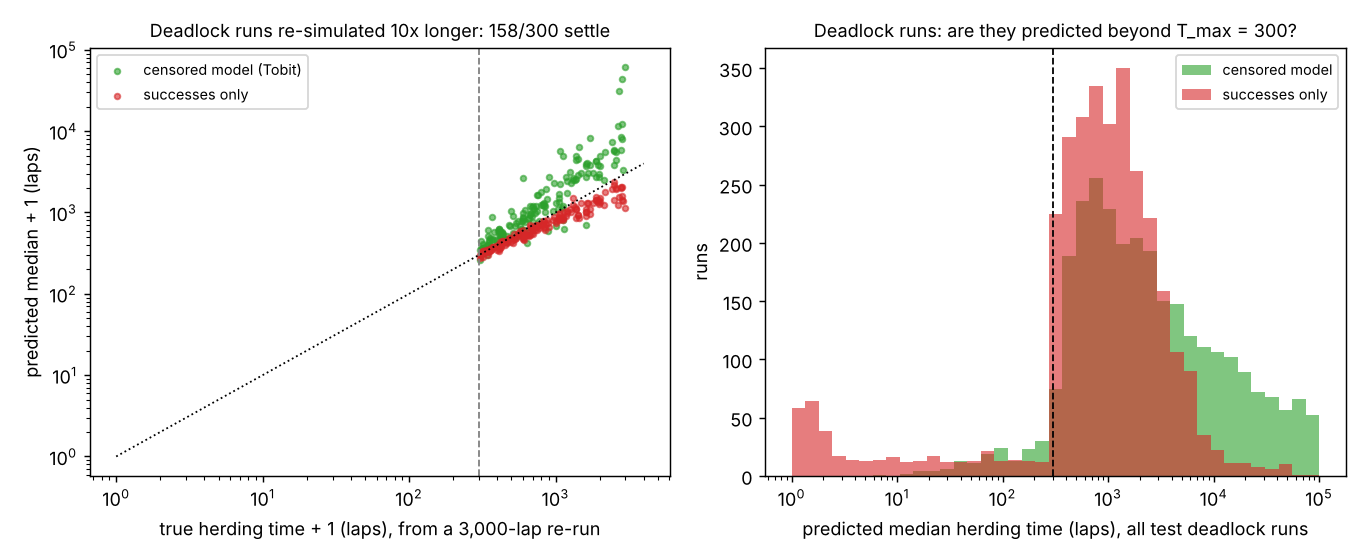
\includegraphics[width=\columnwidth]{censored/censored.png}
\caption{Deadlock runs re-simulated $10\times$ longer. Left: reliability of $P(\text{settles within 3{,}000 laps})$.
Right: predicted vs true herding time of those that settle.}
\label{fig:cens}
\end{figure}

\subsection{Unseen flock sizes: a set kernel}
Hand-made summaries lose information about individual evaders. We also compare runs directly as sets with
$K(A,B)=k_g(g_A,g_B)\,[k_e(e_{0A},e_{0B})+\tfrac{1}{|S_A||S_B|}\sum_{u\in S_A,v\in S_B}k_e(u,v)]$, where $g$ are six global
parameters, $e_0$ the tracked evader and $S$ the set of other evaders (positions$/\kappa$); the bracket is an inner
product of kernel mean embeddings~\cite{muandet2017}, valid for any set sizes. With an SVM and 8{,}000 training runs:
random split 93.6\,\% (hand features 93.0\,\%); trained on $N\le4$, tested on $N=5,6$: \textbf{93.8\,\%} (hand features
90.0\,\%). The set kernel does not degrade on larger flocks.

\subsection{Unsupervised regimes}
PCA and a GMM (BIC) on start features do not recover the classes (ARI 0.08), but on trajectory shapes the clusters are
95\,\% pure and the first two components form one arm per class (Fig.~\ref{fig:reg}): the labels are natural
regimes, and predicting them from the start requires supervision.
\begin{figure*}[t]
\centering
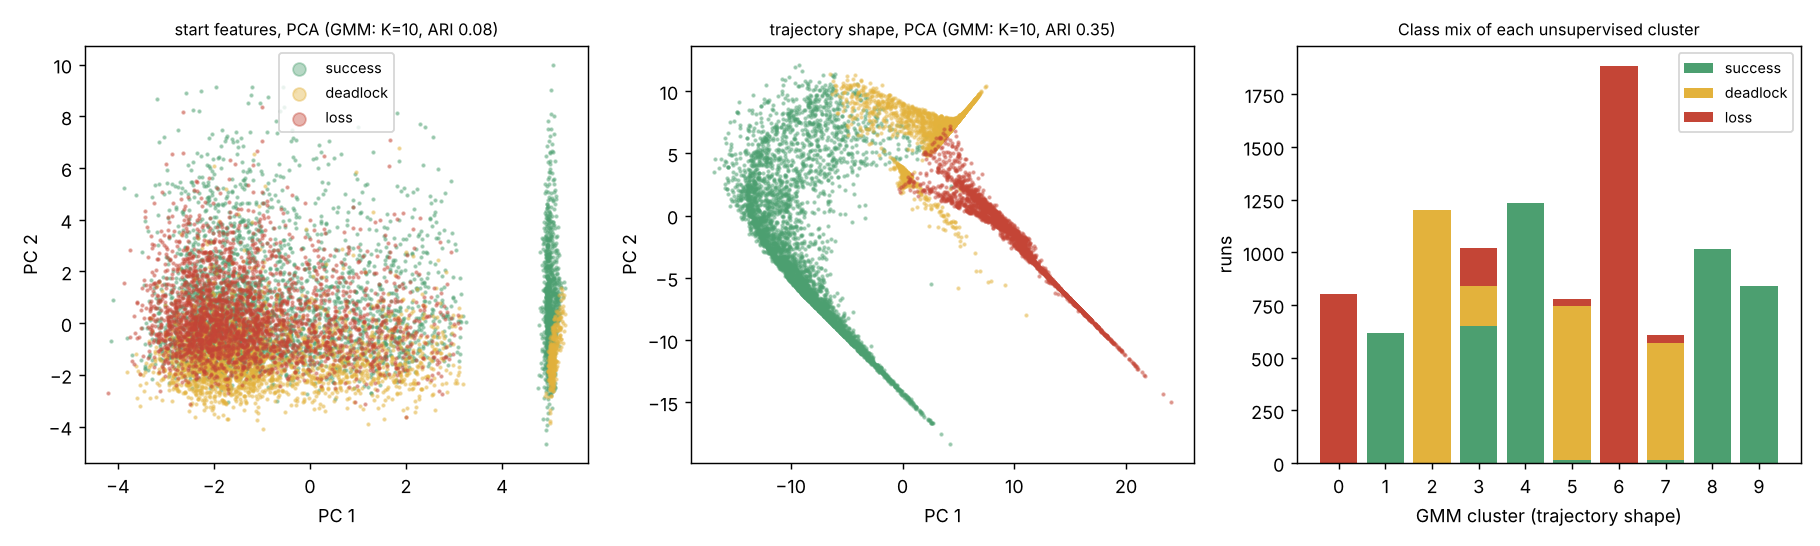
\includegraphics[width=0.92\textwidth]{regimes/regimes.png}
\caption{PCA of start features (left) and of trajectory shapes (middle), coloured by outcome; class mix of the GMM
clusters of trajectory shapes (right).}
\label{fig:reg}
\end{figure*}

\subsection{Risk-aware active learning}
\begin{figure*}[t]
\centering
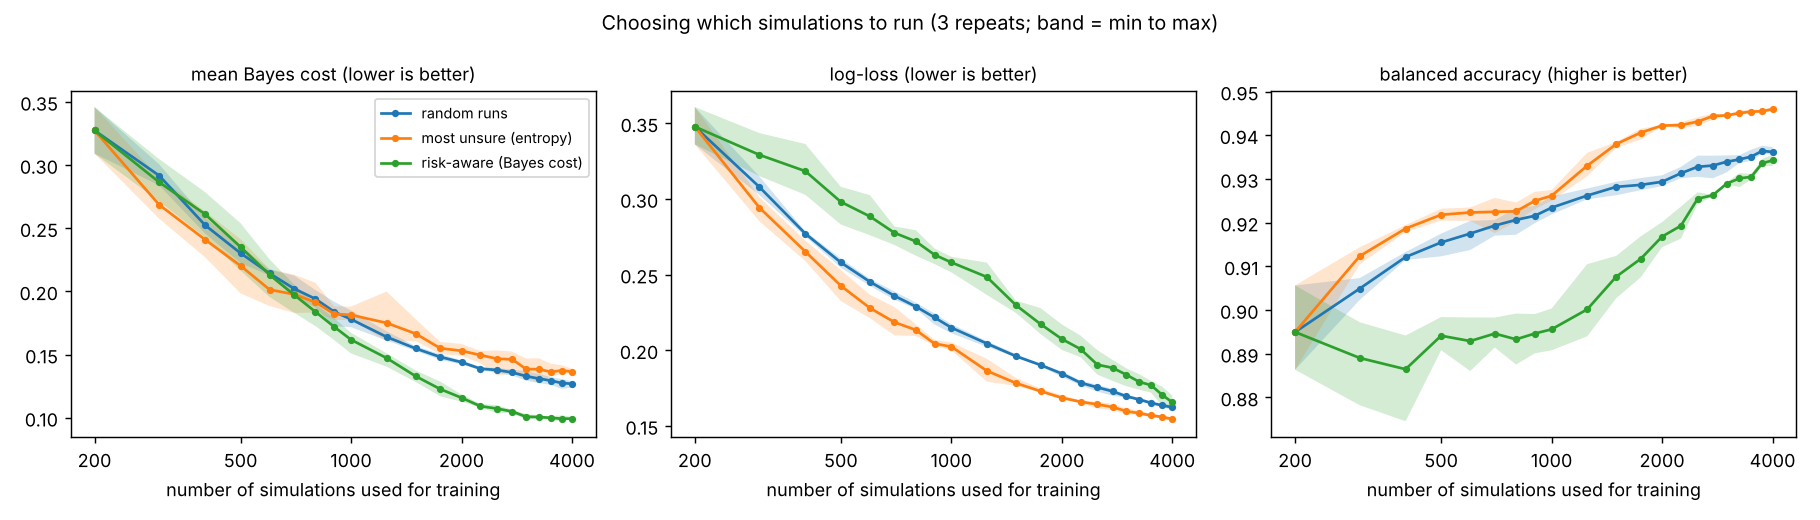
\includegraphics[width=0.92\textwidth]{novelty/active.png}
\caption{Quality vs number of simulations for three acquisition rules (3 repeats; bands = min to max).}
\label{fig:active}
\end{figure*}
Fig.~\ref{fig:active}: risk-aware sampling reaches the decision cost of random sampling at 4{,}000 runs with 1{,}750
(2.3$\times$ fewer) and ends 22\,\% lower (0.099 vs 0.127). Entropy sampling reaches random's accuracy with 1{,}500
runs and ends best in accuracy (0.946), yet its decision cost is \emph{worse} than random (0.137): what to simulate
should follow the decision the model is for.

\subsection{Using the model to choose the pursuer settings}
For 300 held-out multi-evader flocks we let each strategy choose $(q,\beta)$ on a $15\times15$ grid and simulate the
choice (Table~\ref{tab:ctrl}). A theory-guided rule (choose $q$ so that $a=4$, $\beta=1$) never loses an evader.
Maximising the GP's $P(\text{success})$ gives more successes (exact McNemar $p=0.002$) but loses evaders in 3\,\% of
flocks ($p=0.004$). The risk-aware choice---maximise $P(\text{success})$ subject to $P(\text{loss})\le1\,\%$, then the
shortest predicted time from the cure model---matches the theory's zero losses (success 81.7 vs 83.3\,\%, $p=0.06$) and
herds faster: on the 245 flocks where both succeed, median 6 vs 14 laps, faster in 88\,\% (Wilcoxon $p=9\times10^{-24}$).
\begin{table}[t]
\centering
\caption{Simulated outcome of the settings chosen by each strategy (300 flocks).}
\label{tab:ctrl}
\begin{tabular}{lcccc}
\toprule
strategy & success & deadlock & loss & median $T_h$\\
\midrule
random (dataset) & 38.0 & 31.0 & 31.0 & 18.5\\
fixed default & 61.7 & 9.0 & 29.3 & 37\\
theory ($a=4$) & 83.3 & 16.7 & \textbf{0.0} & 15\\
GP, max $P(\text{success})$ & \textbf{86.7} & 10.3 & 3.0 & 6\\
GP-safe, $P(\text{loss})\le1\%$ & 81.7 & 18.3 & \textbf{0.0} & \textbf{6}\\
\bottomrule
\end{tabular}
\end{table}

\begin{figure}[t]
\centering
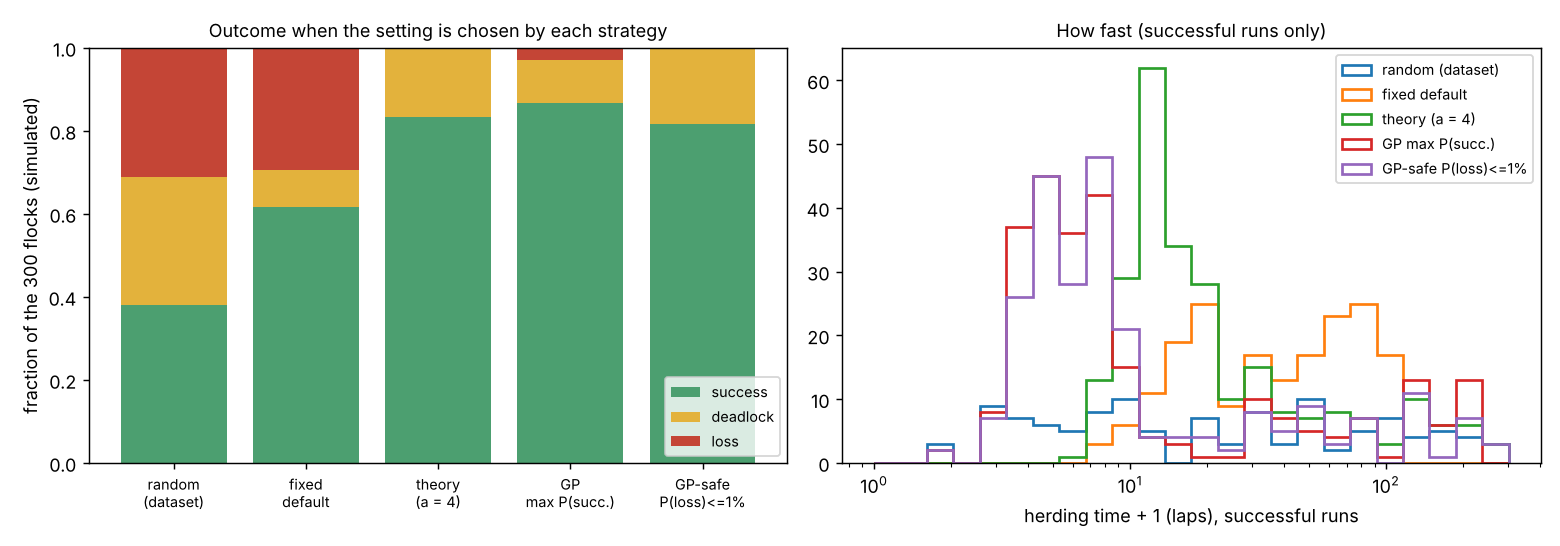
\includegraphics[width=\columnwidth]{control/control.png}
\caption{Outcome (left) and herding time (right) of the settings chosen by each strategy, every choice simulated.}
\label{fig:ctrl}
\end{figure}

\subsection{Theory comparison}
For the circle law we re-solve the paper's Lyapunov-ellipse problem~\cite{singh2024cdc,davison1971} (start from the
Lyapunov-equation solution, optimise the shape, check $\dot V<0$ on dense grids) and compare it with the true region
from a $90\times90$ grid of simulated starts. The certificate is always correct (no false positives) but covers only
0.5\,\% ($\gamma=0.01$) to 3.7\,\% ($\gamma=0.3$) of the truly converging starts (Fig.~\ref{fig:theory}). The reason
is a nearly undamped rotation at the ring (Jacobian eigenvalues $\approx-0.005\pm1i$ at $\gamma=0.01$): a quadratic
Lyapunov function stops decreasing very close to it. Our certified ellipse is smaller than the one drawn
in~\cite{singh2024cdc}; along its limiting direction $\dot V$ indeed turns positive at $0.08R$.
For the arXiv law, Fig.~\ref{fig:map} and the theory-rule baseline show the analogous gap.
\begin{figure*}[t]
\centering
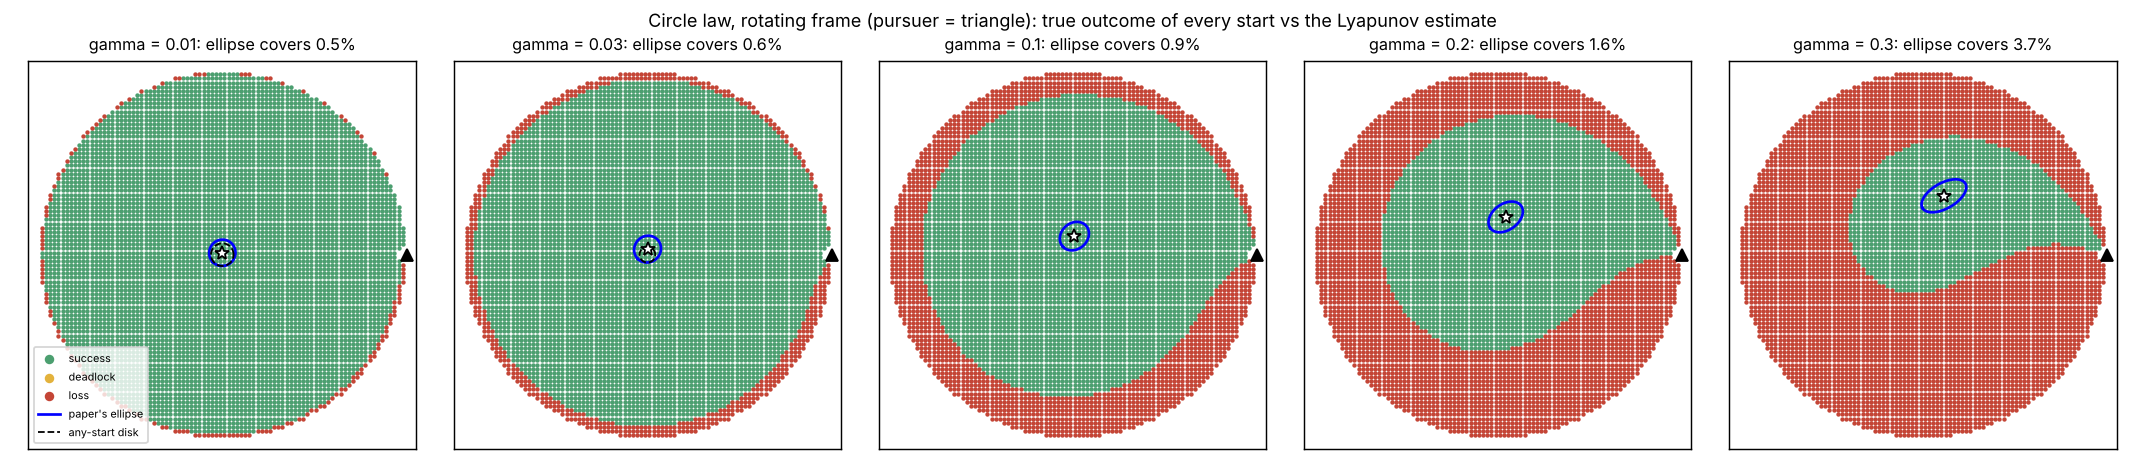
\includegraphics[width=0.92\textwidth]{theory/circle.png}
\caption{Circle law, rotating frame: simulated outcome of every start (green: converges, red: lost) and the
Lyapunov-ellipse certificate (blue).}
\label{fig:theory}
\end{figure*}

\section{Conclusion}
The outcome and duration of single-pursuer herding are predictable from the start with calibrated uncertainty, far
beyond what the local theory certifies: the proven region covers a few percent of the true one, and evaders are lost
where the stability condition holds. Two lessons carry beyond herding. First, censored outcomes hide structure: a
cure model turns ``not finished'' into ``slow'' versus ``stuck'' and predicts it beyond the horizon. Second, both data
collection and decisions should be driven by the cost of the worst mistake: risk-aware active learning needs 2.3$\times$
fewer simulations for the same decision quality, and risk-aware setting selection keeps zero losses while herding
faster. Limits: all results are in simulation; labels depend on $T_{\max}$ and tolerances; exact GPs were limited to
4{,}000 training runs; the cost matrix is a design choice. Future work: switching pursuer laws and noisy sensing.

\section*{Acknowledgment and AI use}
An AI assistant (Claude Code) was used, as allowed in the course, for code, experiments and drafting under the
author's direction; all numbers come from the scripts in the project repository and every choice was checked by the
author.

\bibliographystyle{IEEEtran}
\bibliography{refs}
\end{document}
